\documentclass[12pt,3p]{article}

%This is arxiv version%

%\ifCLASSINFOpdf
%\else
%\fi

\usepackage[english]{babel}
\usepackage{float, color}
\usepackage{graphicx,epstopdf}
\usepackage{amsmath,amssymb,amsfonts,mathrsfs} %subfigure
\usepackage{multicol,subcaption}
\usepackage{comment}
\usepackage{cite}
\usepackage{adjustbox}
\usepackage{pdflscape}
\usepackage{array}
\usepackage{booktabs}
\usepackage{tabularx,ragged2e,booktabs}
\usepackage{amsthm}
\usepackage{hyperref}
\usepackage{setspace}
\usepackage[utf8]{inputenc}
\usepackage{algorithm}
\usepackage{algorithmic}
%\usepackage[linesnumbered,lined,ruled,vlined]{algorithm2e}
%\hypersetup{
%    colorlinks=true,
%    linkcolor=blue,
   % filecolor=magenta,      
%    urlcolor=blue,
%}

\newtheorem{theorem}{Theorem}
%\newtheorem{proof}{Proof}
\newtheorem{corollary}{Corollary}
\newtheorem{statement}{Statement}
\newtheorem{lemma}{Lemma}
%\usepackage{mathtools}

%\pagestyle{headings}
%\setcounter{page}{1}
%\pagenumbering{arabic}


%\usepackage{lineno}
\usepackage[switch]{lineno}
\usepackage[absolute,showboxes]{textpos}

%\setlength{\TPHorizModule}{\paperwidth}\setlength{\TPVertModule}{\paperheight}
%\TPMargin{5pt}

%define \copyrightstatement command for easier use


%\newcommand{\copyrightstatement}{
%    \begin{textblock}{0.41}(0.08,0.93)    % tweak here: {box width}(leftposition, rightposition)
%         \noindent
%         \footnotesize
%         \copyright  2017 licensedusgovmixed ASONAM '17, July 31 - August 03, 2017, Sydney, Australia 978-1-4503-4993-2/17/07 15.00 http://dx.doi.org/10.1145/3110025.3110063
%    \end{textblock}
%}

%\makeatletter
%\def\@IEEEpubidpullup{8\baselineskip}
%\makeatother
%
\begin{document}

%\title{Identify Influential Nodes using h2-index}
%\title{Identify Influential Nodes using h2-index and Hill-Climbing based approach to hit the Most Influential Nodes}
%\title{Identify Influential Nodes using h2-index and Hill-Climbing based approach to hit Top Nodes}

\title{Estimating Shell-Index in a Graph with Local Information}


\author{%
  Akrati Saxena*\\akrati.saxena@iitrpr.ac.in
  \and S. R. S. Iyengar*\\sudarshan@iitrpr.ac.in
  \and *Department of Computer Science and Engineering,\\ Indian Institute of Technology Ropar, India
  }
\date{}

\maketitle

\begin{abstract}
For network scientists, it has always been an interesting problem to identify the influential nodes in the given network. K-shell decomposition method is a widely used method which assigns a shell-index value to each node based on its influential power. The k-shell method requires the global information of the network to compute the shell-index of a node that is not feasible for large-scale real-world dynamic networks. In the present work, we propose a method to estimate the shell-index of a node using local information. We further use hill-climbing based approach to hit the top-ranked nodes in a small number of steps.
%show that the shell-index value of a node can be estimated using its $h^2-index$ which can be computed using local neighborhood information. We further show that $h^2-index$ has better monotonicity and correlation with the spreading power of the node than the shell-index. 

%In real-world applications, it is always required to identify the influential nodes using local information without having the entire network. We show that the top-ranked nodes can be identified in a small number of steps using the hill-climbing approach based random walks.

\end{abstract}


%\IEEEpeerreviewmaketitle

\section{Introduction}

%what is core-periphery

Hierarchical organization of networks gives birth to the core-periphery structure. The concept of the core-periphery structure was first proposed by Borgatti and Everett \cite{borgatti2000models} in 2000. The core is a densely connected nucleus of the network that is surrounded by sparsely connected periphery nodes. Core nodes are highly connected with each other and also highly connected with periphery nodes. Authors proposed an algorithm to detect core-periphery structure based on the adjacency matrix division, such that the number of edges is maximum among core nodes that is preceded by the number of edges between core and periphery, and periphery nodes have very less number of edges among themselves. The complexity of the proposed matrix division method is very high, and so, it is not feasible for large-size real-world networks. Carmi et al. used k-shell decomposition algorithm to identify core-periphery structure in Internet network and classify the network into three categories \cite{carmi2007model}. %This is the first paper that uses k-shell decomposition algorithm to identify core-periphery structure. 


%what is kshell

The K-shell decomposition method was proposed by Seidman and is widely used to identify core nodes in unweighted networks \cite{seidman1983network}. This is a well-known method in social network analysis to identify the tightly knit group of influential core nodes. This algorithm works by recursively pruning the nodes from lower degree to higher degree. First, we recursively remove all nodes of degree 1, until there is no node of degree 1. All these nodes are assigned shell-index $k_s=1$. In the next step, we remove all the nodes of degree 2 if any. While pruning the degree 2 nodes, new nodes having degree 2 or less can be generated and will also be removed in the same iteration. All these nodes will be assigned shell-index $k_s=2$. Similarly, nodes of degree 3, 4, 5,... are pruned step by step. When we remove nodes of degree $k$, if there appears any node of degree less than $k$, it will also be removed in the same step. All these nodes are assigned shell-index $k$. This method thus divides the entire network into shells and assigns a shell-index to each node. The shell-index increases as we move from the periphery to core and the higher shell-index represents the higher coreness. The innermost shell has the highest shell-index $k_{max}$ and is called nucleus of the network. Vladimir Batagelj et al. proposed an order $O(m)$ algorithm to compute the coreness of all nodes, where $m$ is total number of edges in the network \cite{batagelj2011fast}.


%why kshell is important

Many studies have shown that core nodes are highly influential nodes in a network. In the entire paper, by influential node we mean the node having the highest spreading power. In this work, the spreading/influential power of the nodes is computed using SIR spreading model; please refer section~\ref{secsir} for more information. Kitsak et al. \cite{kitsak2010identification} showed that if the infection is started from a core node, it will spread faster than if it is started from any periphery node. Saxena et al. showed the importance of core nodes in information diffusion on the networks having meso-scale structures \cite{saxena2015understanding}. The results show that the information becomes viral once it hits the core nodes and it is spread into multiple communities through the core. Pei and Maske studied the correlation of various centrality measures with the influential power of the nodes on an online social community called LiveJournal and observed that shell-index is an effective centrality measure to identify the most influential nodes \cite{pei2013spreading}. They further extend their study for different types of networks like Twitter, Facebook, and scientific publishing in the American Physical Society, and observe the similar results \cite{pei2014searching}.

%why kshell approximation is required

Shell-index is a good centrality measure to denote the influential power of the node, but it has its disadvantages. Firstly, to compute the shell-index of a node using k-shell decomposition method, we need the entire network as it is a global centrality measure.  With time the size of real-world networks is growing very fast. It is not feasible to collect the entire network to identify the influential power of a node. So, we need faster methods that can estimate the influential power of a node using local neighborhood information. 

Secondly, shell-index assigns the same index values to many nodes which actually might have different influential power \cite{zareie2018hierarchical, wang2016fast, zeng2013ranking}. Zeng et al. modified k-shell decomposition method and proposed a mixed degree decomposition (MDD) method which considers both the residual degree and the exhausted degree of the nodes while assigning them index values \cite{zeng2013ranking}. Liu et al. proposed an improved ranking method that considers both the k-shell value of the node and its distance with the highest k-shell value nodes \cite{liu2013ranking}. The proposed method computes the shortest distance of all nodes with the highest k-shell nodes, so, it has high computational complexity. Liu et al. showed that in real-world networks some core-like groups are formed which are not true-core \cite{liu2015improving}. The nodes in these groups are tightly connected with each other but have very few links outside. Based on this observation, authors filtered out redundant links which have low diffusion power but supports non-pure core groups to be formed, and then apply k-shell decomposition methods. Authors show that the coreness computed on this new graph is a better metric of influential power and it is highly correlated with spreading power computed using SIR model in the original graph. 

%kshell hybrid method
Researchers also have proposed hybrid centrality measures by combining the k-shell with other existing centrality measures. Hou et al. introduced the concept of all-around score to find influential nodes \cite{hou2012identifying}. All around score of a node can be defined as, $Score=\sqrt{\left \| d \right \|^2 + \left \| C_B \right \| ^2 +\left \| k_s \right \|^2 }$, where $d$ is the degree, $C_B$ is the betweenness centrality, and $k_s$ is the shell-index of the node. The degree takes care of local connectivity of the node, betweenness takes care of shortest paths that represent global information, and k-shell represents the position of the node with respect to the center. The total time complexity of the complete process is $O(nm)$, as it depends on the complexity of betweenness centrality that has the highest complexity. Basaras et al. proposed a hybrid centrality measure based on degree and shell-index and showed that it works better than the traditional shell-index \cite{basaras2013detecting}. Bae and Kim proposed a method where the centrality value of a node is computed based on the shell-index value of its neighbors; it thus considers both degree and shell-index value of the nodes \cite{bae2014identifying}. The results show that the proposed method outperforms other methods in the scale-free networks with community structure. Tatti and Gionis proposed a graph decomposition method that considers both the connectivity as well as the local density while the k-shell decomposition method only considers the connectivity of the nodes \cite{tatti2015density}. The running time of the proposed algorithm is $O(|V|^2|E|)$. They further proposed a linear-time algorithm that computes a factor-2 approximation of the optimal decomposition value. All the proposed centrality measures have better monotonicity but all these measures require global information of the network to be computed, and so, they are not favorable in large-scale networks.
%Researchers have also shown that the nodes belonging to the same shell index can have different influential powers \cite{zeng2013ranking, liu2013ranking}.
%Eidsaa and Almaas \cite{eidsaa2013s} extended K-shell decomposition method and proposed S-shell decomposition method for weighted networks.


%what we do in part 1 where we approximate kshell using h2index, we show that h2index is as good as kshell

Lu et al. showed the relationship between degree, h-index \cite{hirsch2005index}, and coreness of a node \cite{lu2016h}. They show that the h-index family of a node converges to the coreness of the node. In this work, we show that shell-index value of a node can be estimated using its $h^2-index$ that can be computed using local neighborhood information of the node. We study the correlation of shell-index and $h^2-index$ with the spreading power of a node and observe that $h^2-index$ have good correlation with the spreading power and can be used in real-world networks to identify the influential nodes. We further show that $h^2-index$ has better monotonicity than the shell-index. 
%In real-world networks, the influential power of a node is measured by using the spreading model. In these models, we start spreading the infection from one node and see how far it goes. To measure the 

%Lu et al. showed the relationship between degree, H-index \cite{hirsch2005index}, and coreness of a node \cite{lu2016h}. In real world networks, it is observed that the coreness is highly correlated with H-index. H-index family of a node is represented as $H(u) = (h_u^{(0)}, h_u^{(1)}, .... , h_u^{(l)})$, where $l$ is the distance of the farthest node from $u$. $h_u^{(0)}$ is the zero order h-index of the node that is equal to the degree of node $u$, $h_u^{(0)} = k_u$. $h_u^{(i)}$ index of a node is calculated using $h_v^{(i-1)}$ index of its neighbors, where $v \epsilon \Gamma(u)$. If we calculate H-index family of a node then it converges to coreness of the node. This method provides us a new perspective to understand the coreness of a node. In k-shell decomposition method we compute coreness using recursive removal of the nodes but in this method, coreness is computed using an iterative procedure.

% what we do in part 2 where we hit the highest h2index node using local random walk

In most of the real world applications, we need to identify highly influential nodes to spread the information without having the global information of the network. Gupta et al. \cite{gupta2016pseudo} proposed Hill-Climbing approach based on the shell-index of the nodes to hit the code nodes. The proposed algorithms cannot be applied in real-world applications as the shell-index is a global parameter and not available locally. We modify the proposed algorithms for $h^2-index$ and the results show that the highest $h^2-index$ nodes can be identified in very less number of steps. We further observe that the subgraph having all the highest $h^2-index$ nodes is connected and we can identify all top-ranked nodes once a node having the highest $h^2-index$ is found. The detailed algorithm and results are discussed in Section~\ref{sec2}.

%section description

%In the present work, we predict the coreness (shell index) of a node using local information. Efficiency of the proposed method is calculated using the modular difference of the actual and predicted coreness. Simulation results show that there is very less error in the predicted coreness value. As per the best of our knowledge, this is the first work of its kind. 
The rest of this paper is organized as follows. In Section~\ref{relwork} we discuss the related literature. Section~\ref{prelim} covers the preliminary definitions. In Section~\ref{section1}, we discuss the estimation of shell-index using $h^2-index$ and experimental results. In Section~\ref{sec2}, we discuss hill-climbing based approachs to identify the top-ranked nodes using local information and their simulation on real-world networks. Section~\ref{conclusion} concludes the paper followed by the future directions.

\section{Related Work}\label{relwork}

% influential nodes and centrality measure

In recent years, the problem of identifying influential nodes has attracted researchers from different areas like computer science, epidemiology, biology, statistics, etc. Researchers have defined various centrality measures to compute the importance of a node based on its characteristics and the given application context. These centrality measures can be categorized as local centrality measures and global centrality measures. Centrality measures that can be computed using local neighborhood information of the node are called local centrality measures like degree centrality \cite{shaw1954some}, h-index \cite{hirsch2005index}, semi-local centrality \cite{chen2012identifying} etc. The centrality measures that require the entire network for their computation are called global centrality measures like closeness \cite{sabidussi1966centrality}, betweenness \cite{freeman1977set}, eigenvector \cite{stephenson1989rethinking}, shell-index \cite{seidman1983network}, PageRank \cite{brin1998anatomy} etc. The computational complexity of global centrality measures is very high, and it depends on the network size.

%kshell is a good measure of influential power: kitsak work
The use of a specific centrality measure to identify important nodes is highly application dependent. Recently Kitsak et al. showed that shell-index is highly correlated with the spreading power of a node \cite{kitsak2010identification}. These results have been supported by many other studies that show that the core nodes are highly influential and the information flows into multiple communities through the core \cite{saxena2015understanding, gupta2016modeling}.


%kshell extensions
Initially, k-shell decomposition method was defined for unweighted undirected networks, but recently it has been extended to different types of networks. Garas et al. extended k-shell method to identify core-periphery structure in weighted networks \cite{garas2012k}. They define the weighted degree that considers both the degree as well as the weights of the connected edges. Then the weighted degree is used while applying the k-shell decomposition method. Eidsaa et al. also proposed a method to identify core-periphery structure in weighted networks where they only consider the strength of the nodes while pruning them in each iteration \cite{eidsaa2013s}. The strength of a node is defined as, $s_i=\sum_{j \epsilon \Gamma (i)} W_{ij}$, where $W_{ij}$ denotes the weight of an edge connecting nodes $i$ and $j$. Wei et al. proposed an edge-weighting k-shell method where they consider both the degree as well as the edge-weights and the edge weight is computed by adding the degree of its two end points \cite{wei2015weighted}. The importance of both of these parameters can be set using a tuning parameter which varies from 0 to 1. If it is set to 0, then the complete importance is given to edge-weights, and if it is set to 1, then the complete importance is given to the degree of the node.
%In weighted networks, node strength\footnote{Strength of a node can be defined as, $s_i=\sum_{j \epsilon \Gamma (i)} W_{ij}$, where $W_{ij}$ denotes the weight of an edge connecting nodes $i$ and $j$.} is used instead of its degree to apply K-shell method and it assigns a shell index to each node. 

%kshell related work
Real-world networks are highly dynamic, and it will not be feasible to recompute the shell-index of each node for every single change in the network. Li et al. proposed a method to update the shell-index value of the affected nodes whenever a new edge is added or deleted from the network \cite{li2014efficient}. Jakma et al. proposed first continuous, distributed method to compute shell-index in dynamic graphs \cite{jakma2012distributed}. Pechlivanidou et al. proposed a distributed algorithm based on MapReduce to compute the k-shell of the graph \cite{pechlivanidou2014mapreduce}. Montresor et al. proposed an algorithm to compute k-shell in live distributed systems \cite{montresor2013distributed}. They further show that the execution time of the algorithm is bounded by $1+\sum_{u \in V}[d(u)-k_s(u)]$ and it gives 80 percent reduction in execution time on the considered real-world networks. Dasari et al. proposed a k-shell decomposition algorithm called ParK that reduces the number of random access calls and the size of working set while computing the shell-index in larger graphs \cite{dasari2014park}. They further proposed a faster algorithm which involves parallel execution to compute the k-shell in larger graphs. Sariyuce et al. proposed the first incremental k-core decomposition algorithms for streaming networks \cite{sariyuce2013streaming}. They show that the proposed method has million times speed-up than the original k-shell method on a network having 16 million nodes.
%Miorandi et al. \cite{miorandi2010k} proposed methods to rank nodes based on coreness in real world dynamic networks. 

 
%Karwa et al. proposed a method to generate all graphs for a given shell-index sequence \cite{karwa2017statistical}.


%kshell applications



%Kshell has wide applications in literature and have 
K-shell method has been widely used in literature to study different networks. 
Catini et al. used shell-index to identify clusters in PubMed scientific publications \cite{catini2015identifying}. To identify the clusters, a graph is created where the nodes are the publications, and there is an edge between two nodes if the distance between the locations of the corresponding researchers is less than the threshold. In the experiments, authors have taken the threshold 1 km. Based on the k-shell decomposition authors categorize the cities into monocore and multicore. Later on, the journal impact factors are used to quantify the quality of research of each core. Results show that k-shell decomposition method can be used to identify the research hub clusters.
%geographical location of the universities/research labs

Core-periphery structure has been studied in the wide variety of networks like financial network \cite{fricke2015core, barucca2016disentangling}, human-brain network \cite{bassett2013task, park2013structural}, nervous system of C. elegans worm \cite{chatterjee2007understanding}, Blog-networks \cite{obradovic2009journey}, collaboration network \cite{leydesdorff2013international, hu2008visual}, protein interaction networks \cite{luo2009core}, Communication network of software development team \cite{crowston2006core, amrit2010exploring, setia2012peripheral, cataldo2008communication}, Hollywood collaboration network \cite{cattani2014insiders}, language network \cite{fedorenko2014reworking}, youtube social interaction network \cite{paolillo2008structure}, metabolic networks \cite{zhao2007modular} etc. Researchers have proposed evolving models to generate synthetic networks having core-periphery structure \cite{saxena2016evolving, adeniji2017generative}. Karwa et al. proposed a method to generate all graphs for a given shell-index sequence \cite{karwa2017statistical}.

%identify core node using local walk

With time the size of real-world networks is increasing exponentially, so, it is not feasible to collect the entire network to study its global properties. Researchers have focussed to propose fast and efficient methods to identify the influential nodes and their ranking in the given network \cite{saxena2017global}. Gupta et al. proposed local information based methods to hit the core nodes quickly \cite{gupta2016pseudo}. 
%In the present work, we  In real-world applications, we are interested in computing the influential rank of a node based on the given centrality measure using minimum information. 
Saxena et al. have proposed fast methods to estimate the degree rank of a node using power-law degree distribution \cite{saxena2015rank, saxena2015estimating} and sampling techniques \cite{saxena2017observe, saxena2017degree}. In \cite{saxena2017fast}, authors proposed heuristic methods to fast estimate the closeness rank of a node. 
%observe that the reverse closeness centrality rank versus closeness centrality follows the sigmoid curve. They use this observation to propose a heuristic method to estimate the closeness rank of a node in $O(m)$ time complexity that is a huge improvement over the classical ranking method having the time complexity $O(n.m)$, where n and m represent the total number of nodes and edges respectively. 
Once the shell-index value is estimated using local information, we aim to propose methods to directly estimate the influential rank of a node without computing the influential value of all nodes. The proposed idea is discussed in detail under Future Directions.
%In \cite{saxena2017afaster}, authors pro closeness rank of the nodes.

% Gupta et al. proposed Hill-Climbing based approaches to hit the code nodes using the shell-index of the node. The proposed algorithms can not be applied in real world applications as the shell-index is a global parameter and not available locally.

\section{Preliminaries}\label{prelim}

%\subsection{kshell Decomposition Method}



\subsection{H-Index}\label{hindex}

The h-index of a node $u$ ($h-index(u)$) is $h$ if $h$ of its neighbors have degree at least $h$ and there is no subset of $h+1$ neighbors where each node belonging to that subset have the degree at least $h+1$.

%define h2index also
The $h^2-index$ of a node $u$ ($h^2-index(u)$) is computed by taking its $h-index$ based on the $h-index$ of its neighbors and not their degrees.

Note: The h-index of a list $l$ ($h-index(l)$) is $h$ if $h$ is the highest number such that $h$ entries of the list are equal to or greater than $h$.

%Note: In this paper, h-index of a list $l$ ($h-index(l)$) computes the $h-index$ of the given list $l$, and h-index of a node $u$ ($h-index(u)$) computes the $h-index$ of the node $u$ based on the degree of its neighbors.

\subsection{SIR Model}\label{secsir}

We use the Susceptible-Infected-Recovered (SIR) spreading model to simulate the spreading process on real-world networks and to compute the spreading power of each node. In SIR model a node can be in three possible states: $1.$ S (susceptible), $2.$ I (infected), and $3.$ R (recovered). Initially all nodes in the susceptible mode except a node which is infected and spread the infection in the network. An infected node will infect each of its susceptible neighbor with probability $\lambda$. If the neighbor gets infected, its status is changed to Infected. Once an infected node contacts all of its neighbors to infect them, its status is changed to recovered state with probability $\mu$. For generality we set $\mu$ = 1. Recovered nodes will neither be infected anymore nor infect others, and they remain in the R state until the spreading stops. 

Initially, we infect a single node, and all other nodes are susceptible. Then the infection starts spreading from the seed node to the others through links. The spreading process stops when there is no infected node in the network. The number of recovered nodes is considered the spreading power or spreading capability of the original node. 
%The proportion of recovered nodes M when spreading stops is considered as the spreading capability, or spreading efficiency, of the origin node.

We execute the SIR model 100 times from each node and take the average of the spreading power to compute the final spreading power of the node. The infection probability is taken as $\lambda > \lambda_c$, where $\lambda_c=\left \langle d \right \rangle/(\left \langle d^2 \right \rangle - \left \langle d \right \rangle)$ is the epidemic threshold computed using mean-field theory, where $d$ represents degree of the node \cite{castellano2010thresholds}.
%We execute the spreading process for 100 times and take the average spreading efficiency of a node as its spreading efficiency.
%As we have discovered that the infection probability will not change the relative spreading efficiency of nodes, we chose
%an infection probability lambda > lambda_c, where lambda_c = <k>/(hk2i − hki) is the epidemic threshold determined from the heterogenous
%mean-field method \cite{castellano2010thresholds}. Under the infection probability of lambda, the final infected populationM is above 0 and reaches a finite but
%small fraction of the network size for most nodes as spreading origins, in the range of 1%-20% \cite{kitsak2010identification}.

\section{Section 1: Shell-Index Estimation}\label{section1}% using $H^2-Index$


The shell-index of a node is the global centrality measure and require entire network for its computation that is not feasible for large-scale dynamic networks. In this section, we discuss the estimation of shell-index using local neighborhood information.
%we show that $h^2-index$ is a good estimation of shell-index. Next, we study the performance of shell-index and $h^2-index$ on real-world networks using monotonicity and SIR spreading model.

\begin{theorem}
The shell-index of a node $u$ can be computed as $k_s(u)=h-index(k_s(v) | \forall v \in ngh(u))$, where $ngh(u)$ is the set of the neighbors of node $u$.
%$S_1, S_2, ... , S_{deg(u)}$ are the shell-indices of the neighbors of $u$ and $S_1 \leq S_2 \leq ... \leq S_{deg(u)}$.
\end{theorem}


\begin{proof}
%\begin{statement}
Let's assume that h-index of $(k_s(v) | \forall v \in ngh(u))$ is $h$ then there are at least $h$ nodes having shell-index equal to or greater than $h$ as per the definition of h-index.
%\end{statement}

Now, we will see how the shell-index of node $u$ will be decided in k-shell decomposition method. In k-shell decomposition method, in $i_{th}$ iteration all those nodes are removed who have exactly $i$ connections with the nodes having the shell-index $i$ or greater that $i$. Thus, the node $u$ will be removed in $h_{th}$ iteration if $h$ of its neighbors have shell-index $h$ or greater than $h$. This is nothing but the $h-index$ of node $u$ based on the shell-indices of its neighbors as defined above. 
\end{proof}

Next, we explain Theorem 1 using examples. The first example is shown in Figure~\ref{exa1}(a) where node $u$ has 8 neighbors having shell-indices 1, 2, 3, 3, 4, 6, 8, and 10. Now, we will see how the shell-index of node $u$ will be determined during the k-shell decomposition method. All the iterations are shown in Figure~\ref{exa1}. In the $1_{st}$ iteration, first of its neighbor will be removed and node $u$ will be left with seven connections with the nodes having the shell-indices greater than $1$, so, the node $u$ will not be removed in the first iteration. In the $2_{nd}$ iteration, its second neighbor will be removed as it has shell-index 2, but still, the node $u$ has six connections with the higher shells, so, it will not be removed. In the third iteration, its 3rd and 4th neighbors will be removed as both of these neighbors have shell-index 3. The node $u$ still has four connections with the higher shells, so it will not be removed. In the 4th iteration, 5th of its neighbor having shell-index 4 will be removed, and now the node $u$ has only three connections with the higher shells, so, as per the k-shell decomposition method, node $u$ will also be removed in 4th iteration. So, the shell-index of node $u$ is 4 that is nothing but the $h-index$ of the shell-indices of its neighbors.

%\begin{figure}[htp]
%  \centering
%    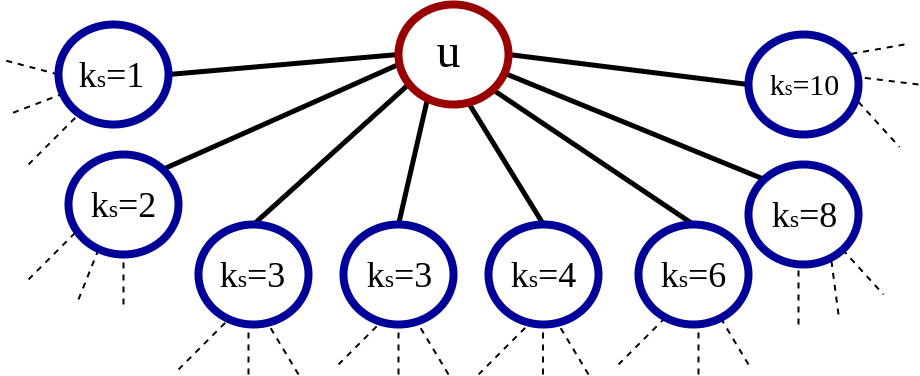
\includegraphics[width=.95\linewidth]{images/kshell_example1.png}
%  \caption{An Example: A subgraph of a network to explain shell-index Computation using shell-indices of neighbors}
%  \label{exa1}
%\end{figure}

%\begin{figure}[!h]
%     \begin{center}
%        \subfigure[Absolute Error]{%
%            \label{fig:first50}
%            \includegraphics[width=0.45\textwidth]{snam/ba1.png}   
%        }\quad%
%        \subfigure[Weighted Error]{%
%           \label{fig:second50}
%           \includegraphics[width=0.45\textwidth]{snam/ba2.png}
%        }
%    \caption{Average Error for BA Networks}
%   \label{baerror}
%   \end{center}
%\end{figure}

\begin{figure}[htp]
  \centering
  \subcaptionbox{Initial subgraph having all connections of node $u$}[.45\linewidth][c]{%
    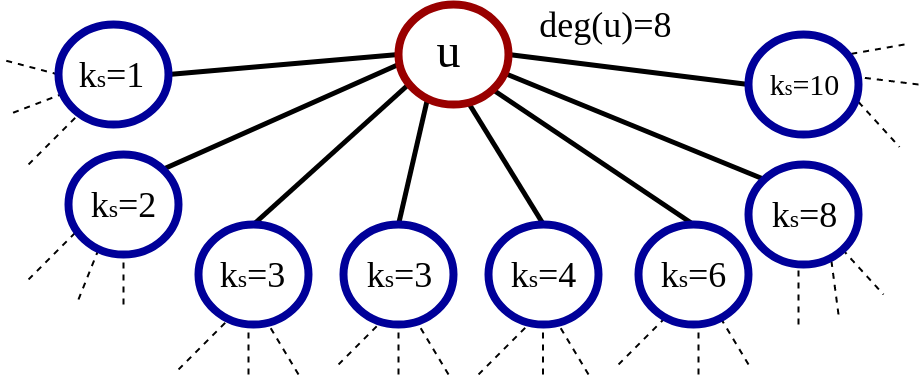
\includegraphics[width=.45\linewidth]{images/kshell_example1_itr0}}\quad
  \subcaptionbox{After Iteration 1}[.45\linewidth][c]{%
    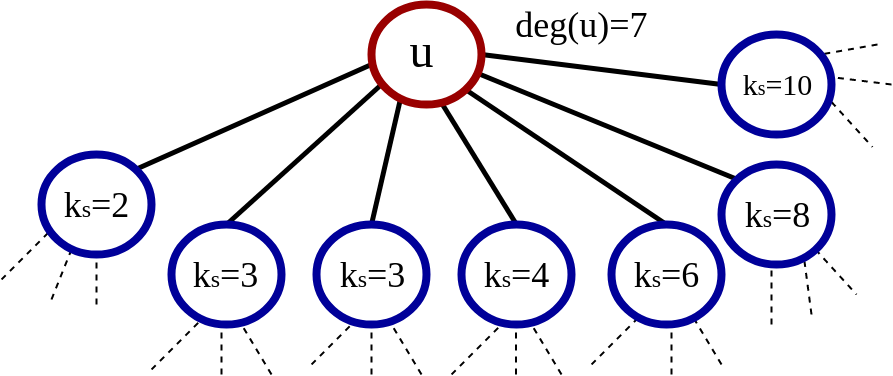
\includegraphics[width=.45\linewidth]{images/kshell_example1_itr1.png}}
  \subcaptionbox{After Iteration 2}[.45\linewidth][c]{%
    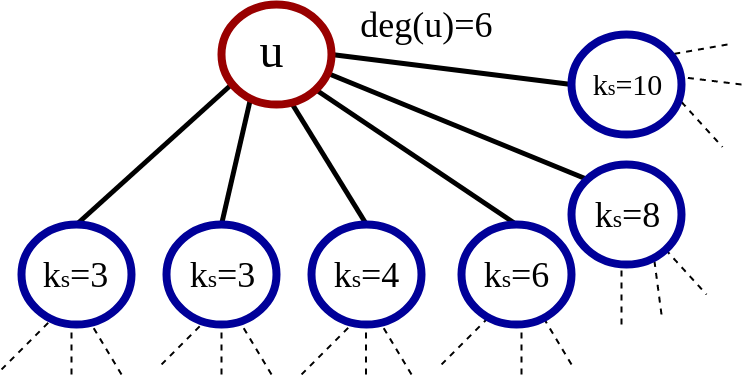
\includegraphics[width=.45\linewidth]{images/kshell_example1_itr2}}\quad
  \subcaptionbox{After Iteration 3}[.30\linewidth][c]{%
    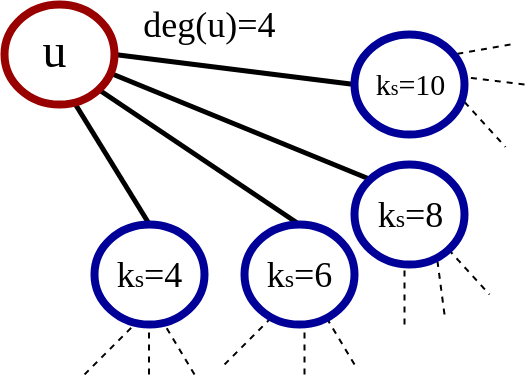
\includegraphics[width=.30\linewidth]{images/kshell_example1_itr3.png}}
  \caption{Example 1: Estimate shell-index of node $u$ while applying k-shell decomposition algorithm}
  \label{exa1}
\end{figure}

%add figures and check grammarly
Similarly, in Figure~\ref{exa2}, node $u$ has degree 7, and the shell-indices of its neighbors are 1, 2, 2, 3, 3, 3, and 5. Now in the 1st iteration of k-shell decomposition method, 1st of its neighbor will be removed. Node $u$ still have 6 connections with the higher shells, so, it will not be removed. In the 2nd iteration, 2nd and 3rd of its neighbors will be removed and node $u$ still have 4 connections with the higher shells, so, it will not be removed. In the 3rd iteration, 4th, 5th, and 6th of its neighbors will be removed, and, now node $u$ have only one connection with the higher shell, so it will also be removed in the same iteration. Thus, it has shell-index 3.

\begin{figure}[htp]
  \centering
    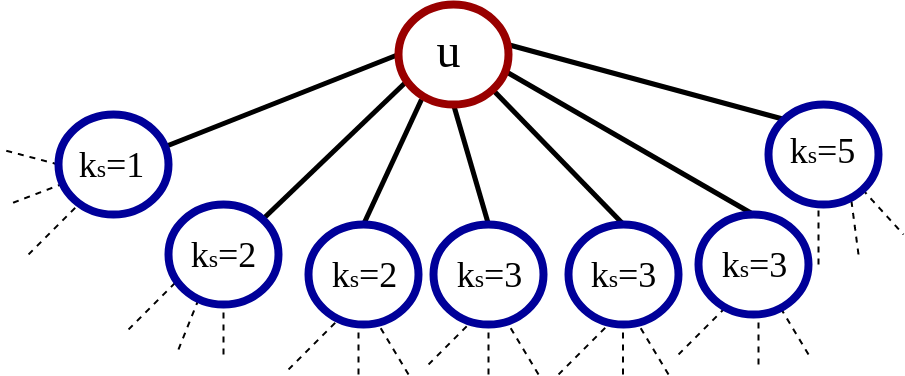
\includegraphics[width=.55\linewidth]{images/kshell_example2.png}
  \caption{Example 2: A subgraph of a network to explain shell-index Computation using shell-indices of neighbors}
  \label{exa2}
\end{figure}

In Figure~\ref{exa3}, node $u$ has degree 6 and the shell-indexes of its neighbors are 10, 11, 11, 13, 15, and 25. In 1st, 2nd,..., 5th iteration, the node $u$ will not be removed as it has 6 connections with the higher shells. In the 6th iteration, node $u$ will be removed as it has degree 6, so, the shell-index of node $u$ is 6, i.e., the h-index of the shell-indices of its neighbors.

\begin{figure}[htp]
  \centering
    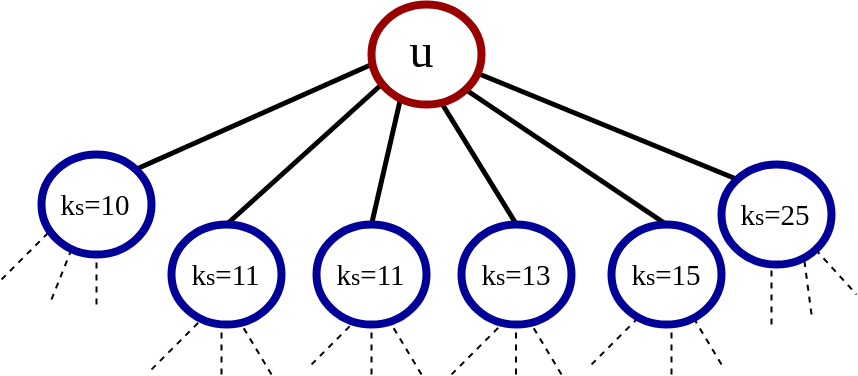
\includegraphics[width=.55\linewidth]{images/kshell_example3.png}
  \caption{Example 3: A subgraph of a network to explain shell-index Computation using shell-indices of neighbors}
  \label{exa3}
\end{figure}

\subsection*{Shell-Index Estimation}

Using Theorem 1, the shell-index of a node can be estimated if the shell-indices of its neighbors are known. But in real life applications, the shell-indices of the neighbors will not be known. We know that the shell-index of a node is bounded above by its degree, $k_s(u) \leq d(u)$. So, to estimate the shell-index of node $u$, we can consider the degrees of its neighbors in place of their shell-indices. This is nothing but the $h-index$ of node $u$ as defined in Section~\ref{hindex}. To further improve the estimation, we consider the $h-index$ of its neighbors as $k_s(v) \leq h-index(v) \leq d(v)$ and this is nothing but the $h^2-index$ of the node. Thus the shell-index of a node can be estimated using its $h^2-index$. Next, we will study the performance of the proposed estimator in real-world networks.

Pseudo-code is given in Algorithm 1, where $ngh(u)$ is the list of the neighbors of node $u$. The proposed estimator can be further improved if we compute the $h^3-index$ of the node but in the results section, we show that $h^2-index$ is itself a good estimator. It can be computed faster and requires less neighborhood information than to compute the $h^3-index$ of the node.
%In our analysis, we use $h^2-index$ to estimate the $shell-index$ and to measure the spreading power of a node.  % and function $h-index(list)$ returns the $h-index$ of the given list. 
 
%we compute the h2-index of node u that is h-index of the h-indexes of its neighbors. 
%compute the h-index of the degrees of its neighbors. This is nothing but the h-index of node u. To better estimate the shell-index, we compute the h2-index of node u that is h-index of the h-indexes of its neighbors. The algorithm is given in algorithm 1. 

\begin{algorithm}
\caption{$Compute\_h^2-index(G,u)$}%Compute $h^2-index$, 
\begin{algorithmic}
\STATE Take a list $ngh\_hindex$, $ngh\_hindex=[\; ]$
\FOR{each $v$ in $ngh(u)$}
\STATE add $h-index(v)$ in $ngh\_hindex$
\ENDFOR
\STATE return $h-index(ngh\_hindex)$
\end{algorithmic}
\end{algorithm}

%\begin{algorithm}
%\caption{$Compute\_h2index(G,u)$}%Compute $h^2-index$, 
%\begin{algorithmic}
%\STATE take a list $ngh\_hindex$, $ngh\_hindex=[\; ]$
%\STATE take a list $ngh\_deg$, $ngh\_deg=[\; ]$
%\FOR{each $v$ in $ngh(u)$}
%\STATE $ngh\_deg=[\; ]$
%\FOR{each $w$ in $nbr(v)$}
%\STATE add $deg(w)$ in $ngh\_deg$
%\ENDFOR
%\STATE add $h-index(ngh\_deg)$ in $ngh\_hindex$
%\ENDFOR
%\STATE return $h-index(ngh\_hindex)$
%\end{algorithmic}
%\end{algorithm}

\subsection{Results and Discussion}

We study the performance of $h^2-index$ versus shell-index on the following real-world networks. 
%The experiments are performed on $1.$ collaboration networks: Astro-Physics, Cond-Mathematics, DBLP, $2.$ social networks: Buzznet, Digg, Facebook, Foursquare, Gowalla $3.$ communication network: Enron, and $4.$ Interaction network: FB-wall is a social interaction network of Facebook users.

\subsection*{Datasets}

\begin{enumerate}
\item \textbf{Astro-Ph:} This is the co-authorship network of ArXiv's Astrophysics (Astro-ph) publications where authors are represented by nodes, and there is an edge between two nodes if the corresponding authors have published together \cite{leskovec2007graph}. It contains 14845 nodes and 119652 edges.

\item \textbf{Buzznet:} Buzznet is a subgraph extracted from a social networking site that is used to share photo, journal, and video \cite{zafarani2009social}. It consists of 101163 nodes and 2763066 edges.

\item \textbf{Cond-Mat:} This is the co-authorship network of ArXiv's condensed matter section \cite{leskovec2007graph}. This dataset covers all papers from January 1993 to April 2003 (124 months). It contains 13861 nodes and 44619 edges.

\item \textbf{DBLP:} This is a coauthorship network extracted from DBLP computer science bibliography, where edge denotes that the autors have common publications \cite{yang2015defining}. This network contains 317080 nodes and 1049866 edges.

\item \textbf{Digg:} This friendship network was extracted from Digg website in 2009 \cite{hogg2012social}. It contains 261489 nodes and 1536577 edges.

\item \textbf{Enron:} This network is the email communication network of the employees of Enron organization from 1999 to 2003 \cite{klimt2004enron}. Nodes of the network are email addresses and there is an edge between two nodes if they have communicated at least once. The dataset has 84384 nodes and 295889 edges. 

\item \textbf{Facebook:} This dataset is an induced subgraph of Facebook \cite{viswanath2009evolution}, where users are represented by nodes and friendships are represented by edges. It contains 63392 nodes and 816831 edges.

\item \textbf{FB-Wall:} This is a network where nodes are Facebook users and there is an edge between two users if any one of them post on the Facebook-wall of other user \cite{viswanath2009evolution}. It contains 43953 nodes and 182384 edges.

\item \textbf{Foursquare:} Foursquare is a location-based social networking software for mobile devices that can be accessed using GPS. This dataset is an induced subgraph of friendships of Foursquare  \cite{zafarani2009social}. It contains 639014 nodes and 3214985 edges.

\item \textbf{Gowalla:} This friendship network is extracted from a location based social network called, Gowalla \cite{cho2011friendship}. This was used to shared the locations among its users. It contains 196591 nodes and 950327 edges.

\end{enumerate}

The experimental results are shown in Table~\ref{sec1results}. First, we compute the monotonicity of shell-index and $h^2-index$. Ideally, if a node has influential power different from other nodes, it should be assigned a unique index value. In k-shell decomposition method, all the nodes which are pruned at one level are assigned the same shell-index value. Researchers have shown that they have different influential power and should have been assigned different values \cite{zareie2018hierarchical, wang2016fast, zeng2013ranking}. So, a good centrality measure will assign the same value to fewer nodes and assign more unique values. This characteristic of the measure can be computed using the monotonicity \cite{bae2014identifying}. This is defined as,

\begin{center}
$M(R)=\left( 1-\frac{\sum_{r \in R}n_r(n_r-1)}{n(n-1)} \right) ^2$
\end{center}

where $R$ denotes the ranking values of all the nodes based on any given centrality measure, $n$ represents the size of $R$ i.e. the number of nodes in our case, and $n_r$ represents the number of nodes having rank $r$. If all nodes have the same rank, the monotonicity $(M)$ of the ranking is 0, and it is not a valid ranking measure. If each node has a unique rank then the monotonicity $(M)$ is 1, and it shows that the given ranking measure is perfect. The results in Table~\ref{sec1results} show that the monotonicity of $h^2-index$ is either same or slightly better than the shell-index. 

Next, we study the correlation of shell-index and $h^2-index$ with the spreading power of the node. The spreading power of a node is computed by executing the SIR model (SIR model is defined in Section~\ref{secsir}) 100 times and taking the average number of infected nodes. In experiments, the infection probability $\lambda$ is taken as $\lambda=\left \langle d \right \rangle/(\left \langle d^2 \right \rangle - \left \langle d \right \rangle) + 0.01$. To study the correlation, we compute Kendall's Tau $(\tau)$, Pearson $(r)$, and Spearman $(\rho)$ correlation coefficients. The results in Table~\ref{sec1results} show that the correlation of $h^2-index$ with the spreading power is either as good as the correlation of shell-index with the spreading power or better.

%we compute pearson and spearman correlation of shell-index and h2-index with the SIR spreading ranks. The results are shown in Table x.

\begin{table*}[htp]
\centering
\caption{Performance of Shell-Index ($k_s$) and $h^2-index$ using monotonicity and SIR spreading model}
\label{sec1results}
\resizebox{\columnwidth}{!}{%
\begin{tabular}{|l|l|l|l|l|l|l|l|l|l|l|l|}
\hline
Network & Ref &  Nodes & Edges & \multicolumn{2}{|c|}{Monotonicity} & \multicolumn{3}{|c|}{$k_s$ vs. SIR} & \multicolumn{3}{|c|}{$h^2-index$ vs. SIR} \\ \hline

	&	&	&	&  $k_s$ & $h^2-Index$ & Kendall &  Pearson & Spearman & Kendall &  Pearson & Spearman \\	\hline
%	&	&	&	&  $k_s$ & $h^2-Index$ & $\tau$ &  $r$ & $\rho$ &  $\tau$ & $r$ & $\rho$ \\	\hline
																			
Astro-Ph	&	\cite{leskovec2007graph}	&	14845	&	119652	&	0.89	&	0.89	&	0.51	&	0.67	&	0.67	&	0.52	&	0.67	&	0.68	\\ \hline
Buzznet	&	\cite{zafarani2009social}	&	101163	&	2763066	&	0.93	&	0.93	&	0.21	&	0.28	&	0.30	&	0.21	&	0.28	&	0.30	\\ \hline
Cond-Mat	&	\cite{leskovec2007graph}	&	13861	&	44619	&	0.75	&	0.76	&	0.55	&	0.69	&	0.69	&	0.56	&	0.70	&	0.70	\\ \hline
DBLP	&	\cite{yang2015defining}	&	317080	&	1049866	&	0.74	&	0.75	&	0.49	&	0.61	&	0.61	&	0.49	&	0.62	&	0.62	\\ \hline
Digg	&	\cite{hogg2012social}	&	261489	&	1536577	&	0.45	&	0.45	&	0.48	&	0.60	&	0.59	&	0.48	&	0.60	&	0.59	\\ \hline
Enron	&	\cite{klimt2004enron}	&	84384	&	295889	&	0.30	&	0.30	&	0.45	&	0.58	&	0.55	&	0.45	&	0.58	&	0.55	\\ \hline
Facebook	&	\cite{viswanath2009evolution}	&	63392	&	816831	&	0.91	&	0.91	&	0.49	&	0.64	&	0.65	&	0.49	&	0.64	&	0.65	\\ \hline
Fb-Wall	&	\cite{viswanath2009evolution}	&	43953	&	182384	&	0.76	&	0.77	&	0.62	&	0.75	&	0.76	&	0.62	&	0.75	&	0.76	\\ \hline
Foursquare	&	\cite{zafarani2009social}	&	639014	&	3214985	&	0.50	&	0.50	&	0.54	&	0.66	&	0.65	&	0.54	&	0.66	&	0.65	\\ \hline
Gowalla	&	\cite{cho2011friendship}	&	196591	&	950327	&	0.73	&	0.74	&	0.59	&	0.71	&	0.72	&	0.59	&	0.71	&	0.72	\\ \hline
																	
\end{tabular}	
}																	
\end{table*}

Next, we study how the correlation of shell-index and $h^2-index$ with the spreading power changes as we vary the infection probability. The results are shown for Astro-physics collaboration network and Facebook wall social interaction network in Figure~\ref{fig2}. The epidemic threshold value ($\lambda_c$) for Astro-Ph and FB-Wall network is 0.02 and 0.04 respectively, so, the considered range of the infection probability is taken $0.05-0.14$, i.e., greater than the $\lambda_c$ for both the networks. The results show that $h^2-index$ has good correlation with varying infection probabilities. 
We also observe that the correlation of both the centrality measures decreases as we increase the infection probability that is not desirable. It helps to conclude that the proposed centrality measure can be further improved using other available local information of the node.

%insert figure here
\begin{figure}[htp]
  \centering
  \subcaptionbox{Astro-Ph Collaboration Network}[.95\linewidth][c]{%
    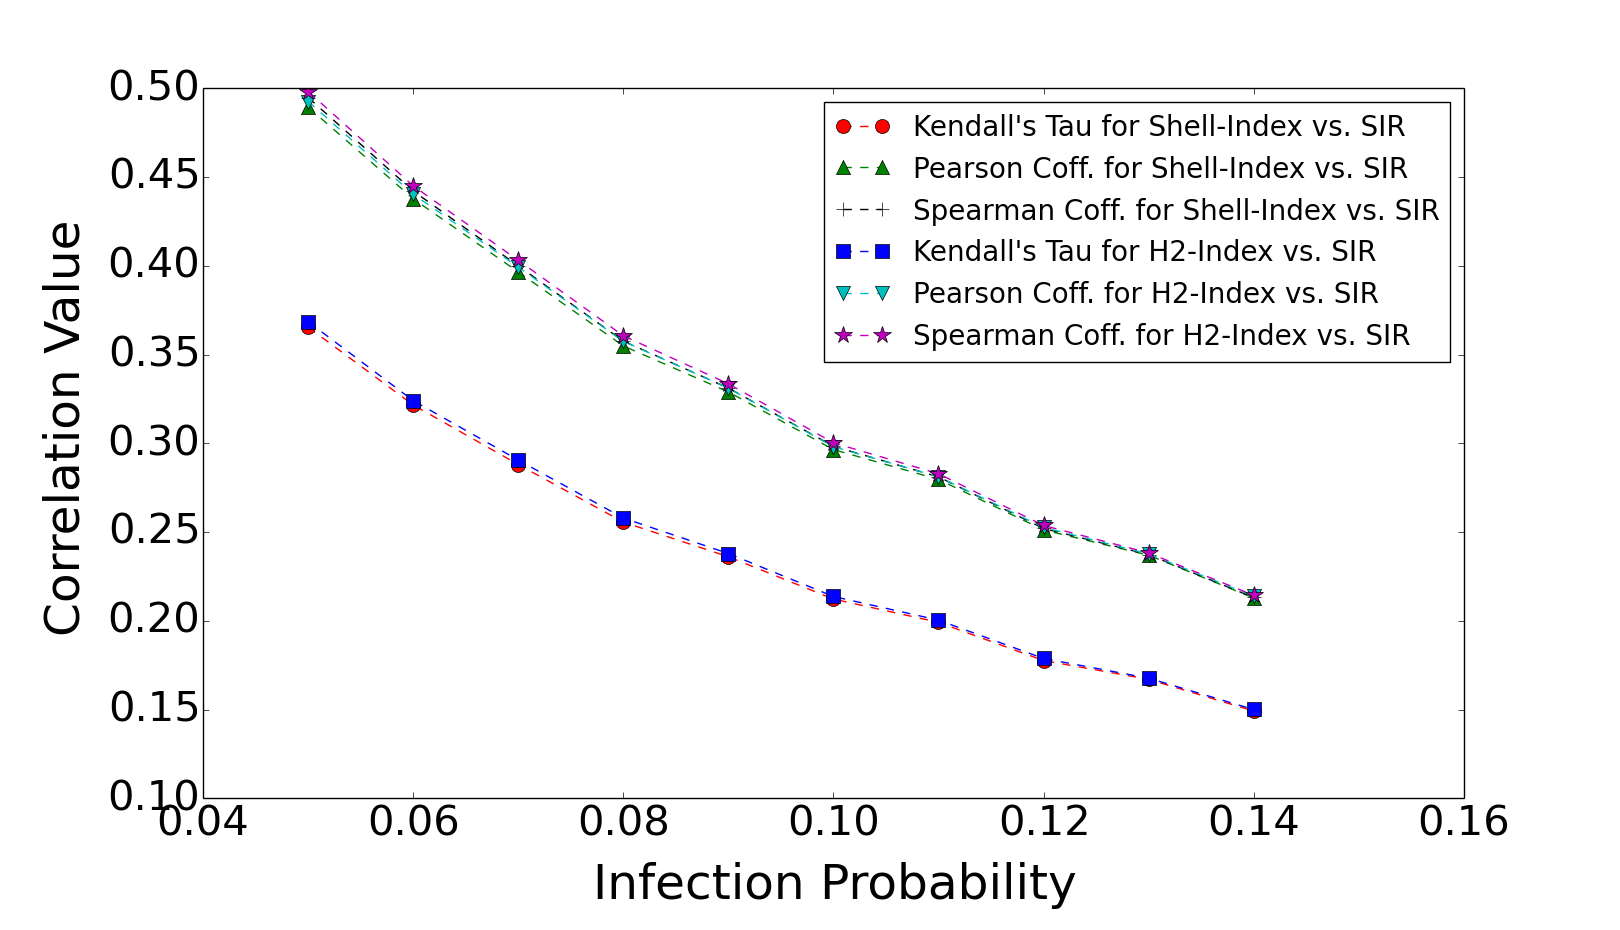
\includegraphics[width=.95\linewidth]{images/astroph1.png}}\quad
  \subcaptionbox{FB-Wall Social Interaction Network}[.95\linewidth][c]{%
    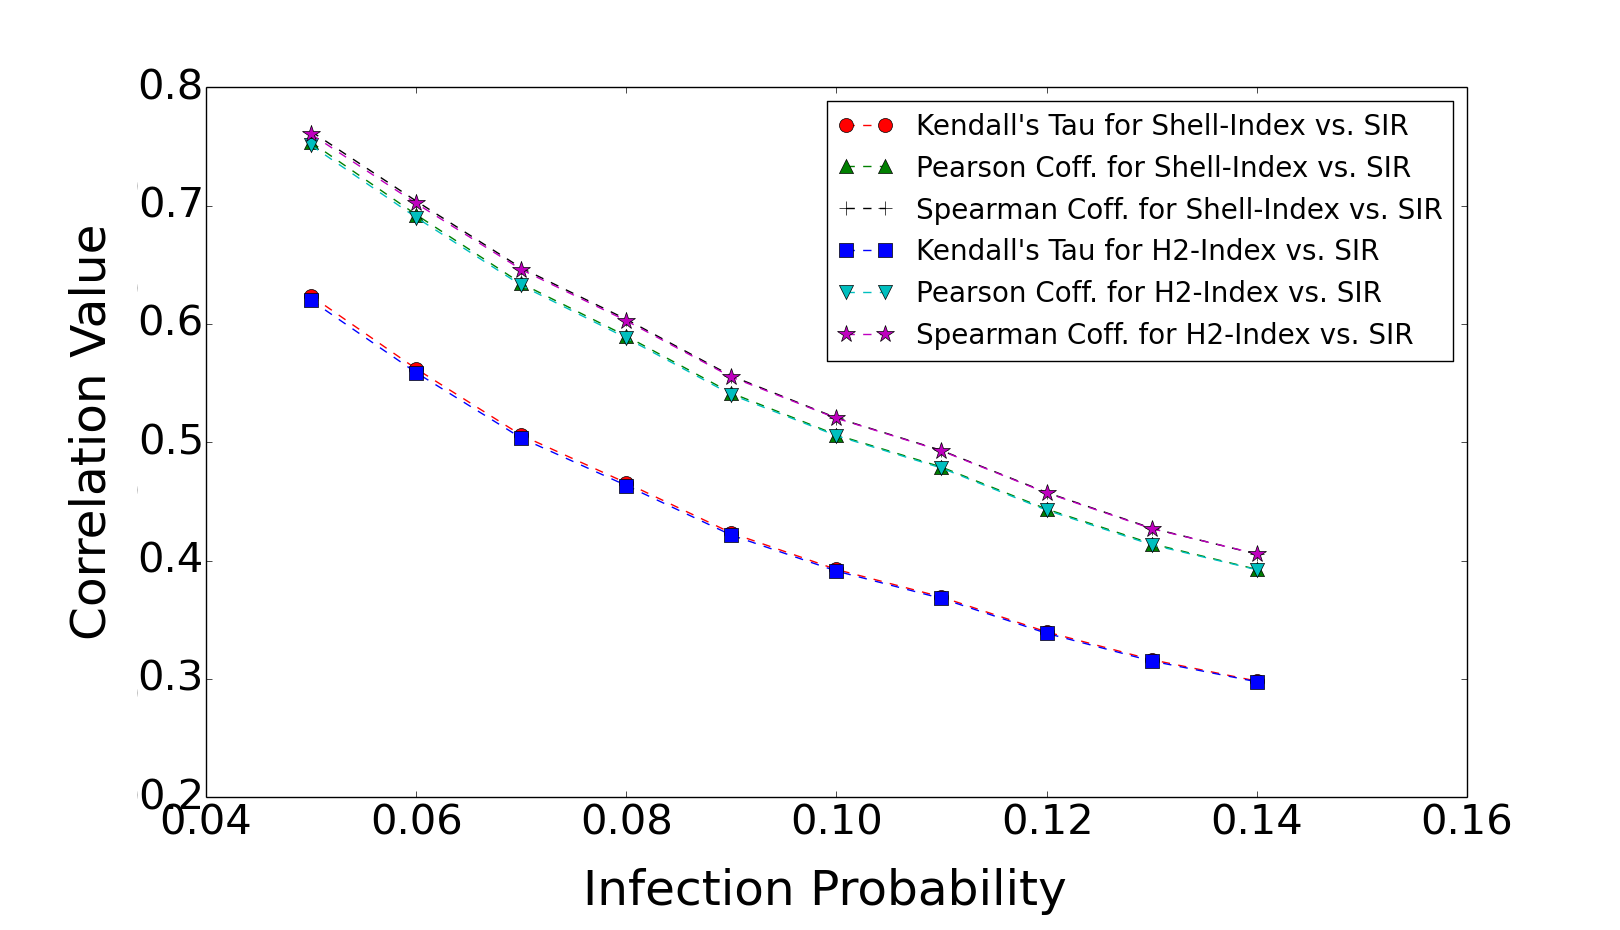
\includegraphics[width=.95\linewidth]{images/fbwall1.png}}
  \caption{Shell-Index and $h^2-index$ correlation with spreading power for varying infection probability a. Astro-Ph and b. FB-Wall network}
  \label{fig2}
\end{figure}

Thus we observe that $h^2-index$ is a better centrality measure than the shell-index in real-world networks. $h^2-index$ has an advantage over shell-index as it is a local centrality measure and can be computed for a node using local neighborhood information without collecting the entire network.

\section{Section 2: Hill-Climbing based approach to Identify Top-Ranked Nodes}\label{sec2}

In many real-life applications, we need to identify top influential nodes to spread the information faster. For example, if a marketing company wants to provide free samples of their products, they would like to find out the influential people in the network who can help them to spread the word faster about their product. Similarly, if someone wants to spread a virus using Internet network, she would like to find out and infect the node having the highest spreading power. 

With time, the size of real-world networks is growing very fast, and it is not feasible to collect the entire network to identify the top influential nodes. So, we need to propose methods to identify these nodes using local information without having the global information. By the global information, we mean the network properties which need the entire network to be computed like network size, average degree, the highest $h^2-index$ of the network, and so on. Researchers have proposed various sampling-based methods to estimate global properties of the network like network size \cite{kurant2012graph}, global clustering coefficient \cite{hardiman2013estimating}, average degree \cite{dasgupta2014estimating}, degree distribution of the network \cite{ribeiro2012estimation}, and so on.

In this work, we have shown that the influential power of a node can be computed using its $h^2-index$, i.e. a local measure. For a given node, even if we compute its $h^2-index$ locally, we do not know how influential this node is in the entire network, and whether this node belongs to the highest influential nodes or not. In \cite{gupta2016pseudo}, Gupta et al. proposed Hill-Climbing based methods that can be used to hit the highest shell-index nodes faster in a network. In the proposed method, the random walker starts from a periphery node and move to one of its neighbor having the highest shell-index until a top node is found. The proposed method cannot be applied in practice as the shell-index is a global centrality measure, but the results show that using the proposed Hill-Climbing based random walk, the most influential nodes can be hit in a very small number of steps.  %Results are shown in Table x and figure x.

We modify the proposed methods to identify the highest $h^2-index$ node in the network. In rest of the paper, the \textit{top-ranked nodes} refer to the nodes having the highest $h^2-index$ in the network. The algorithm is given in Algorithm~\ref{algo2}. The input of the algorithm are $G$, $u$, $k$, and $maxindex$ where $G$ is the given network, $u$ is the seed node from which the crawler starts crawling the network, $k$ is the repeat-count that shows how many times the crawler will restart the walk from a randomly chosen neighbor of the current node if it is stuck to the local maxima, and $maxindex$ is the maximum $h^2-index$ in the given network. A node is called local maxima if its $h^2-index$ is higher than all of its neighbors. The nodes having the highest $h^2-index$ in the network are called global maxima. For the clarification, a local maxima can also be the global maxima. In Algorithm~\ref{algo2}, $ngh(u)$ represents the set of all the neighbors of node $u$. $randomchoice(list)$ function returns a random element from the given list. 

The algorithm works in the following manner. 
%If the input node has the highest $h^2-index$, the algorithm returns that the given node has the highest $h^2-index$ and exits. Otherwise, t
The crawler starts from the given node $u$ and it moves to one of its neighbors that has not been visited before and has the highest $h^2-index$. The crawler keeps moving until it hits the local maxima. If this node has the highest $h^2-index$, the algorithm exits, else the crawler jumps to one of its non-visited neighbors uniformly at random and the repeat-count is increased by one. The same procedure is repeated until the highest $h^2-index$ node is identified or the repeat-count reaches its maximum value. If the algorithm reaches to maximum repeat-count without finding out the highest $h^2-index$, it returns "The algorithm is failed to find out the top-ranked node."  %returns the number of steps and
%The random walker keeps moving until it hits a node who has none of its neighbors having the h2-index more than itself. This is called the local maxima and we note down the number of steps \textit{$initial_steps$} taken by the crawler till now. If this node has highest h2-index, the algorithm returns number of steps and exits, else the crawler jumps to one of its non-visited neighbors uniformaly at random and the repeatcount is increased by one. The same steps are repeated until the highest h2-index node is identified or the repeatcount reaches to its maximum value. If the algorithm reaches to maximum repeatcount without finding out the highest h2-index, it returns "the algorithm is failed to find out top ranked node." 

%\begin{algorithm}[]
%\caption{$IndexBasedHillClimbing(u,G)$}
%Take a list $visited\_nodes$ and $visited\_nodes = []$\;
%\For{$i\leftarrow 1$ \KwTo $k$}{
%Select a node $w$ uniformly at random\;
%Add $closeness\_centrality(G,w)$ in list L\;
%}
%$c'_{mid}$ = average of all values of $L$\;
%Estimate closeness rank of the node using equation \ref{closerank} as, $R_{est}(u)=1 + \frac{n-1}{1+\left(\frac{C(u)}{c'_{mid}}\right)^p}$\;
%Return $R_{est}(u)$\;
%\end{algorithm}

%\begin{algorithm}
%\caption{$IndexBasedHillClimbing(G,u,k)$}
%\label{algo1}
%\begin{algorithmic}
%\STATE Take a list $visited\_nodes$ and $visited\_nodes = [\;]$
%\STATE $num\_of\_steps=0$
%\STATE $repeat\_count=0$
%\STATE $current\_node=u$
%\STATE add $u$ in $visited\_nodes$
%\STATE $flag=True$
%\WHILE{$flag == True$}
%%\STATE $nextnode=argmax_{v \in ngh(current\_node)\; \& \; v\; is\; not\; in\; visited\_nodes}h2-index(v)$
%%\STATE $nextnode=$
%%\STATE $argmax_{v \in ngh(current\_node)\; \& \; v\; \notin visited\_nodes}h^2-index(v)$
%\STATE $next\_node=current\_node$
%\FOR {$each \; v \; in \; ngh(current\_node)$} 
%\IF {$h^2-index(v) \geq h^2-index(next\_node) \; and \; v \notin visited\_nodes$}
%\STATE $next\_node=v$
%\ENDIF
%\ENDFOR
%%\STATE $next\_node=argmax\{h^2-index(v) | v \in ngh(current\_node) \& v \notin visited\_nodes\}$
%\IF {$next\_node == current\_node$}
%\IF {$repeat\_count<k$}
%\STATE $next\_node=$
%\STATE $randomchoice_{v \notin visited\_nodes}ngh(current\_node)$
%\STATE $repeat\_count=repeat\_count+1$
%\ELSE
%\STATE Print "The algorithm is failed to find out the top-ranked node."
%\STATE $flag=False$
%\ENDIF
%\ELSE
%\STATE $current\_node=next\_node$
%\ENDIF
%\STATE add $current\_node$ in $visited\_nodes$	
%\STATE $num\_of\_steps=num\_of\_steps+1$
%\ENDWHILE
%\STATE return $h^2-index(current\_node)$
%\end{algorithmic}
%\end{algorithm}


\begin{algorithm}
\caption{$IndexBasedHillClimbing(G,u,k,maxindex)$}
\label{algo2}
\begin{algorithmic}
\STATE Take a list $visited\_nodes$ and $visited\_nodes = [\;]$
\STATE $num\_of\_steps=0$
\STATE $repeat\_count=0$
\STATE $current\_node=u$
\STATE $next\_node=u$
\STATE add $u$ in $visited\_nodes$
\STATE $flag=True$
\WHILE{$flag == True$}
%\STATE $next\_node=current\_node$
\FOR {$each \; v \; in \; ngh(current\_node)$} 
\IF {$h^2-index(v) \geq h^2-index(next\_node) \; and \; v \notin visited\_nodes$}
\STATE $next\_node=v$
\ENDIF
\ENDFOR
\IF {$next\_node == current\_node$}
\IF {$h^2-index(next\_node) == maxindex$}
\STATE $flag=False$
\ELSIF {$repeat\_count<k$}
\STATE $next\_node=randomchoice_{v \notin visited\_nodes}ngh(current\_node)$
%\STATE $$
\STATE $repeat\_count=repeat\_count+1$
\ELSE
\STATE Print "The algorithm is failed to find out the top-ranked node."
\STATE $flag=False$
\ENDIF
%\ELSE
%\STATE $current\_node=next\_node$
\ENDIF
\IF {$flag==True$}
\STATE add $next\_node$ in $visited\_nodes$	
\STATE $current\_node=next\_node$
\STATE $num\_of\_steps=num\_of\_steps+1$
\ENDIF
\ENDWHILE
\STATE return $h^2-index(current\_node)$
\end{algorithmic}
\end{algorithm}

The proposed method is further modified as shown in Algorithm~\ref{algo3} named $IndexAndDegreeBasedHillClimbing(G,u,k,maxindex)$. In this method, the crawler will move to one of the highest degree nodes among the non-visited neighbors having the highest $h^2-index$. Except this, there is one more change; once the algorithm stuck to local maxima, the crawler moves to one of its non-visited neighbors having the highest degree. The highest degree node has a high probability to be connected with the top-ranked nodes, and so, this algorithm will work faster and better than the first one.

\begin{algorithm}
\caption{$IndexAndDegreeBasedHillClimbing(G,u,k,maxindex)$}
\label{algo3}
\begin{algorithmic}
\STATE Take a list $visited\_nodes$ and $visited\_nodes = [\;]$
\STATE $num\_of\_steps=0$
\STATE $repeat\_count=0$
\STATE $current\_node=u$
\STATE $next\_node=u$
\STATE add $u$ in $visited\_nodes$
\STATE $flag=True$
\WHILE{$flag == True$}
%\STATE $next\_node=current\_node$
\FOR {$each \; v \; in \; ngh(current\_node)$} 
\IF {$h^2-index(v) \geq h^2-index(next\_node) \; and \; v \notin visited\_nodes$}
\STATE $next\_node=v$
\ENDIF
\ENDFOR\
\FOR {$each \; v \; in \; ngh(current\_node)$} 
\IF {$h^2-index(v) == h^2-index(next\_node) \; and \; deg(v) \geq deg(next\_node) \; and \; v \notin visited\_nodes$}
\STATE $next\_node=v$
\ENDIF
\ENDFOR\
\IF {$next\_node == current\_node$}
\IF {$h^2-index(next\_node) == maxindex$}
\STATE $flag=False$
\ELSIF {$repeat\_count<k$}
%\STATE $next\_node=$
%\STATE $randomchoice_{v \notin visited\_nodes}ngh(current\_node)$
\FOR {$each \; v \; in \; ngh(current\_node)$} 
\IF {$deg(v) \geq deg(next\_node) \; and \; v \notin visited\_nodes$}
\STATE $next\_node=v$
\ENDIF
\ENDFOR\
\STATE $repeat\_count=repeat\_count+1$
\ELSE
\STATE Print "The algorithm is failed to find out the top-ranked node."
\STATE $flag=False$
\ENDIF
%\ELSE
%\STATE $current\_node=next\_node$
\ENDIF
\IF {$flag==True$}
\STATE add $next\_node$ in $visited\_nodes$	
\STATE $current\_node=next\_node$
\STATE $num\_of\_steps=num\_of\_steps+1$
\ENDIF
\ENDWHILE
\STATE return $h^2-index(current\_node)$
\end{algorithmic}
\end{algorithm}
%We further modify the algorithm as proposed in \cite{gupta2016pseudo}. In this updated version, the random walker to move one of its neighbors having the highest h2-index and highest degree. The rest of the algorithm is same and the results are shown in table X.



\subsection*{Discussion}

We implement the proposed methods on real-world networks, and the results are shown in Table~\ref{sec2results}. In the experiments, the algorithm is executed from all non top-ranked nodes (the nodes not having the highest $h^2-index$), and the number of steps taken to hit a top-ranked node are averaged to compute the average number of steps. In experiments, the value of repeat-count $(k)$ is set to 50. In Table~\ref{sec2results}, the average and the standard deviation of the number of steps are shown in $Avg(steps)$ and $Std(steps)$ columns. The $Avg(count)$ shows the average of the number of repeat-count that algorithm takes when it is stuck to a local maxima. The $Algo\;Failed(\%)$ shows how many times the algorithm is not succeeded to hit the top-ranked node in the given repeat-count. The algorithm might succeed if we increase the value of repeat-count. %over all iterations

The results show that on an average a top-ranked node can be reached in very few steps (3-213 in the considered datasets), and the average value of the repeat-count is 0-10. The algorithm is failed in very few cases for the repeat-count 50. In the case of $IndexAndDegreeBasedHillClimbing(G,u,k,maxindex)$ Algorithm, the average number of steps and the average repeat-count is reduced but the probability to fail the algorithm is increased in the given repeat-count as the crawler always moves to higher degree nodes and ends up following the same path that leads to stuck to the local maxima. In DBLP network the probability of failure is much higher when we apply degree based hill-climbing approach as the algorithm is mostly stuck to a local maxima due to following the same route and not able to hit the global maxima in the given repeat-count. This highly depends on the network structure and not on its size. %In practice, the crawler can be started from different randomly chosen nodes to increase the probability to hit the top-ranked node. In real-world networks, we do not know the highest h2-index, so, the algorithm needs to be repeated few more times when it is stuck to local maxima to make sure that the returned node by the algorithm has the actual global maxima not the local maxima. 

When we apply this algorithm in practice, we do not know the value of the highest $h^2-index$ ($maxindex$), so, the algorithm needs to be repeated few more times when it is stuck to a local maxima to make sure that the node returned by the algorithm has the actual global maxima and not the local maxima. The results show that a smaller value of $repeat-count$ will suffice the purpose. The methods can be started from few randomly chosen nodes to avoid the local maxima and hit the top-ranked nodes with a high probability.

%add how to modify this algorithm to apply in the practice
%When we apply this algorithm in practice, we do not know the value of the highest h2-index, so, we need to set the repeat-count such that we hit the top ranked node with high probability. We have applied the methods on real-world networks and the results are discussed in the next section. The results show that a small value of the repeat-count will suffice the purpose. The methods can be started from few randomly chosen nodes to avoid the local maxima and hit the top-ranked nodes with high probability.

%the found node having the highest h2-index is the actual global maxima not the local maxima. 

%This might also be the global maxima and the node might be having the highest h2-index in the given network, but we are not sure of it. Now the random walker is moved to one of its neighbor randomly and it keeps moving until it hit the next maxima or it has travelled for $5*initial_steps$, whichever happens later. Then we see how many times the proposed algorithm actually hit the highest h2-index node and how many times the algorithm is stuck to the local maxima. 





\begin{table*}[htp]
\centering
\caption{Results for $IndexBasedHillClimbing(G,u,k,maxindex)$ and $IndexAndDegreeBasedHillClimbing(G,u,k,maxindex)$ Algorithms}
\label{sec2results}
\resizebox{\columnwidth}{!}{%
\begin{tabular}{|l|l|l|l|l|l|l|l|l|l|}
\hline
Network &  Nodes & \multicolumn{4}{|c|}{$IndexBasedHillClimbing(G,u,k,maxindex)$} & \multicolumn{4}{|c|}{$IndexAndDegreeBasedHillClimbing(G,u,k,maxindex)$} \\ \hline

%	&	&  $Avg(steps)$ & $Std(steps)$ & $avg(repeat-count)$ & $Algo\;Failed(\%)$ &  $Avg(steps)$ & $std(steps)$ & $avg(repeat-count)$ & $Algo\;Failed(\%)$ \\	\hline
	
	&	&  $Avg$ & $Std$ & $Avg$ & $Algo$ &  $Avg$ & $Std$ & $Avg$ & $Algo$ \\
	
	&	& $(steps)$  & $(steps)$  & $(count)$ & $Failed(\%)$ & $(steps)$  &$(steps)$  & $(count)$ & $Failed(\%)$ \\	\hline
 
Astro-Ph	&	14845	&	8.66	&	9.82	&	0.37	&	1.21	&	5.70	&	1.40	&	0.00&	3.27	\\ \hline																			
Buzznet	&	101163	&	3.20	&	0.69	&	0.00	&	0.00	&	3.20	&	0.69	&	0.00	&	0.00	\\ \hline

Cond-Mat	&	13861	&	15.55	&	15.46	&	2.27	&	1.39	&	9.95	&	4.88	&	0.18	&	11.58	\\ \hline

DBLP	&	317080	&	213.13	&	84.89	&	9.79	&	5.45	&	118.76	&	5.34	&	0.00	&	79.60 \\ \hline
																			
Digg	&	261489	&	4.09	&	1.50	&	0.02	&	0.03	&	4.03	&	0.85	&	0.00	&	0.15	\\ \hline
																			
Enron	&	84384	&	5.08	&	0.97	&	0.00	&	0.00	&	5.07	&	0.93	&	0.00	&	0.04	\\ \hline																							
Facebook	&	63392	&	6.06	&	1.90	&	0.30	&	0.00	&	5.99	&	1.80	&	0.31	&	0.02	\\ \hline																					
FB-Wall	&	43953	&	9.04	&	4.48	&	0.59	&	0.00	&	8.65	&	4.12	&	0.48	&	0.04	\\ \hline
																	
Foursquare	&	639014	&	10.84	&	0.38	&	0.00	&	0.00	&	10.84	&	0.38&	0.00	&	0.00	\\ \hline
																			
Gowalla	&	196591	&	4.33	&	4.17	&	0.15	&	0.02	&	3.92	&	1.32	&	0.03	&	0.22	\\ \hline
																	
\end{tabular}	
}																	
\end{table*}


%\begin{table*}[h]
%\centering
%\caption{Error in the Estimated Ranking}
%\label{results}
%%\resizebox{\columnwidth}{!}{%
%\begin{tabular}{|l|l|l|l|l|l|l|l|l|l|}
%\hline
%Network &  Nodes & \multicolumn{4}{|c|}{Algo1} & \multicolumn{4}{|c|}{Algo2} \\ \hline
%
%	&	&  Steps Avg. & Steps Std. & Count & Algo Failed &  Steps Avg. & Steps Std. & Count & Algo Failed \\	\hline
%																			
%actor	&	374511	&	4.14	&	1.79	&	0.01	&	0.04	&	4.12	&	1.52	&	0	&	0.07	\\ \hline
%																			
%enron	&	84384	&	5.08	&	0.97	&	0	&	0	&	5.07	&	0.93	&	0	&	0.1	\\ \hline
%																			
%brightkite	&	56739	&	4.9	&	1.96	&	0.04	&	0.11	&	4.82	&	1.32	&	0	&	0.76	\\ \hline
%																			
%facebook final	&	63392	&	6.06	&	1.9	&	0.3	&	0	&	6	&	1.81	&	0.3	&	0.1	\\ \hline
%																			
%as skitter	&	771892	&	5.49	&	1.57	&	0.13	&	0	&	5.25	&	1.15	&	0.13	&	0	\\ \hline
%																			
%fb wosn	&	43953	&	9.04	&	4.48	&	0.59	&	0	&	9.48	&	5.09	&	0.62	&	0.35	\\ \hline
%																			
%foursquare	&	639014	&	10.84	&	0.38	&	0	&	0	&	10.84	&	0.38	&	0	&	0	\\ \hline
%																			
%petster	&	148826	&	4.52	&	0.62	&	0	&	0	&	4.51	&	0.62	&	0	&	0.01	\\ \hline
%																			
%buzznet	&	101163	&	3.2	&	0.69	&	0	&	0	&	3.2	&	0.69	&	0	&	0	\\ \hline
%																			
%digg	&	261489	&	4.09	&	1.5	&	0.02	&	0.03	&	4.03	&	0.85	&	0	&	0.63	\\ \hline
%																			
%epinion	&	75877	&	3.85	&	0.93	&	0.01	&	0	&	3.82	&	0.83	&	0	&	0.38	\\ \hline
%																			
%caida	&	26475	&	3.55	&	0.71	&	0	&	0	&	3.54	&	0.69	&	0	&	0.05	\\ \hline
%																			
%twitter	&	81306	&	3.64	&	0.77	&	0	&	0	&	3.64	&	0.77	&	0	&	0	\\ \hline
%																			
%hyves	&	1138245	&	5.7	&	1.77	&	0.08	&	0	&	5.29	&	1.4	&	0.04	&	0	\\ \hline
%																			
%fb 4k	&	4039	&	115.1	&	60.02	&	19.15	&	5.52	&	83.48	&	39.87	&	9.65	&	1.88	\\ \hline
%																			
%cond mat	&	13861	&	15.55	&	15.46	&	2.27	&	1.39	&	11.24	&	7.84	&	0.32	&	12.01	\\ \hline
%																			
%dblp	&	317080	&	213.13	&	84.89	&	9.79	&	5.45	&	135.25	&	20.42	&	0.29	&	62.8	\\ \hline
%																			
%slashdot	&	82168	&	3.97	&	0.73	&	0	&	0	&	3.97	&	0.71	&	0	&	0.14	\\ \hline
%																			
%youtube	&	1134885	&	5.07	&	2.04	&	0.06	&	0.05	&	4.94	&	1.1	&	0	&	1.33	\\ \hline
%																			
%gplus	&	107614	&	4.04	&	0.51	&	0	&	0	&	4.04	&	0.51	&	0	&	0	\\ \hline
%																			
%gowalla	&	196591	&	4.33	&	4.17	&	0.15	&	0.02	&	t	&	t	&	t	&	t	\\ \hline
%																			
%euall	&	224832	&	4.81	&	1.92	&	0.02	&	0	&	4.76	&	0.55	&	0	&	0.11	\\ \hline
%																			
%lastfm	&	1191805	&	4.7	&	0.79	&	0	&	0	&	4.7	&	0.79	&	0	&	0	\\ \hline
%																			
%topology	&	34761	&	4.37	&	0.66	&	0	&	0	&	4.37	&	0.66	&	0	&	0.01	\\ \hline
%																			
%livemocha	&	104103	&	3.49	&	0.8	&	0.04	&	0	&	3.45	&	0.7	&	0.04	&	0	\\ \hline
%																			
%Astro-ph	&	14845	&	8.66	&	9.82	&	0.37	&	1.21	&	8	&	7.14	&	0.01	&	2.65	\\ \hline
%
%																	
%\end{tabular}	
%%}																	
%\end{table*}

%The proposed methods can be further improved by computing the h2-index of the neighbors who have higher degree than the h2-index of the current node. A node having the degree below than the current node can never have the h2-index higher than the current node, so it is not required to be considered. This further fasten up the proposed method. 

The proposed methods can be further improved by only computing the $h^2-index$ of the neighbors that can be considered for the next step of the crawler instead of computing the $h^2-index$ of all of its neighbors. A node having the degree lower than the $h^2-index$ of the current node cannot have the $h^2-index$ higher than the current node, so, all such neighbors can be discarded. This further fastens up the proposed method. 

%We can further improve the proposed method, if we use only the h-index for the initial walk and once the local maxima is hit we can use h2-index. It will further fasten up the method.

We further observe that in real-world networks, the subgraph of all top-ranked nodes (the highest $h^2-index$ nodes) is connected. So, once we hit one top-ranked node, all top-ranked nodes can be identified. All these nodes can be used to spread the information faster in the network.
%It can further fasten the information spreading process.% can be used to spread the information. %all the considered

\section{Conclusion}\label{conclusion}

In this work, we have shown that $h^2-index$ is a good estimation of shell-index and can be used to identify influential nodes in real-world networks. 
%We further compare the performance of $h^2-index$ and shell-index using monotonicity and SIR spreading model and 
We also observed that $h^2-index$ has better monotonicity than the shell-index and has better correlation with the spreading power of the nodes.
%In real life applications, we need to identify influential nodes using local information without having the entire network. 
Next, we used Hill-Climbing based methods to hit the top-ranked nodes in the given network. The results show that a top-ranked node can be found in very less number of steps using local information. In very few cases, the walk is trapped at the local maxima and does not hit the top-ranked node. We further observed that all top-ranked nodes form a connected subgraph and once we find one top-ranked node, all the most influential nodes can be identified. In future, we would like to propose mathematical bound to compute the required number of steps to hit a top-ranked node in the given scale-free real-world network.

\section{Future Directions}

%This study further opens up various new research directions that can be looked at.
%
%\subsection*{Estimate the Influential Rank using Local Information}

%In the present work, we show that $h^2-index$ is a good centrality measure that can be used to identify the influential nodes. It has an advantage as it is a local centrality measure and can be computed for a node using its local neighborhood information. $h^2-index$ assigns an index value to each node that represents its influential power. But it gives no idea about how influential this node is with respect to the other nodes as we don't know what the minimum or maximum influential powers in the given network is and how these values vary among the nodes. 
In many real-life applications, users are interested to know the relative importance of the node that can be measured using the rank of the node. The classical method to compute the rank of a node, will compute the index value of all the nodes and will compare them to get the rank of the interested node. The time complexity of the proposed method is very high as it computes the centrality value for all the nodes and its space complexity is also high as it requires the entire network. In future, we are planning to propose fast and efficient methods that can directly estimate the $h^2-index$ rank of a node using local information without computing the centrality value of all the nodes. 

We observe that percentile rank versus $h^2-index$ follows a unique pattern in all real-world networks as shown in Figure~\ref{fig1}. The percentile rank of a node is computed as $PercentileRank(u)=\frac{n-R(u)+1}{n}*100$, where $n$ is the network size and $R(u)$ is the rank of node $u$ based on its $h^2-index$ value in the given network. We study this curve and find that 4-parameters logistic equation better fits the curve. The equation of the curve is given as $PercentileRank(u) = n + \frac{1-n}{1+\left( \frac{h^2-index(u)}{C_{mid}}\right) ^p}$, where $C_{mid}$ represents the $h^2-index$ value of the middle ranked node in the network, and $p$ denotes slope of the logistic curve at the middle point (also called hill's slope). The plots are shown for Astro-physics and FB-Wall interaction network in Figure~\ref{fig1}, where black line shows the actual percentile rank of the nodes and the red line shows best fit for the 4-parameter logistic equation. The best fit curve is plotted using scaled Levenberg-Marquardt algorithm \cite{more1978levenberg} with 1000 iterations and 0.0001 tolerance. Once we estimate the parameters of the equation, the rank of a node can be computed in $O(1)$ time without computing the index values of all the nodes. A similar approach has been used to estimate the closeness rank of a node in $O(m)$ time that is a huge improvement over the classical ranking method having the time complexity $O(n.m)$ where $n$ and $m$ represent the total number of nodes and edges respectively \cite{saxena2017afaster}.

%insert figure here
\begin{figure}[htp]
  \centering
  \subcaptionbox{Astro-Ph Collaboration Network}[.9\linewidth][c]{%
    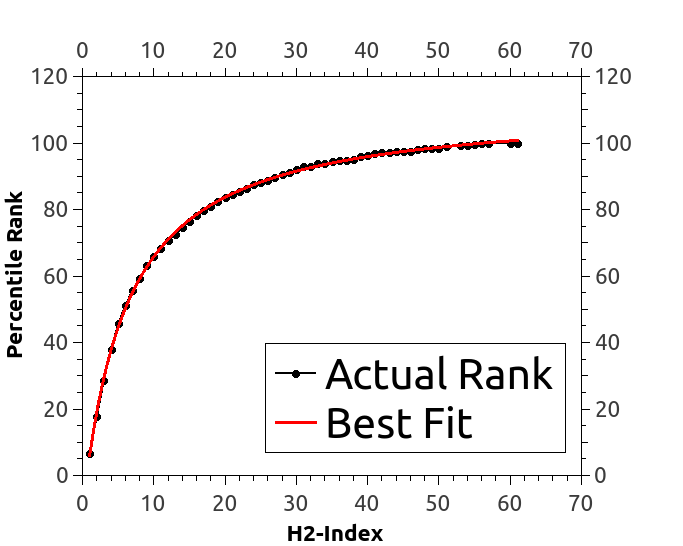
\includegraphics[width=.9\linewidth]{images/astroph_qti.png}}\quad
  \subcaptionbox{FB-Wall Social Interaction Network}[.9\linewidth][c]{%
    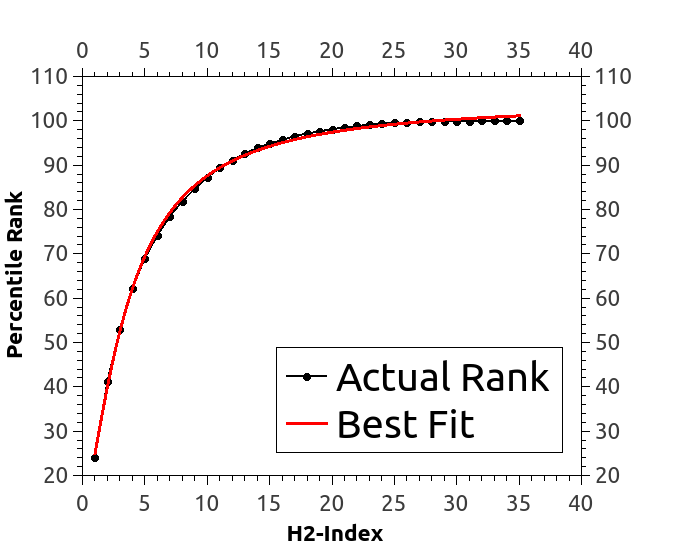
\includegraphics[width=.9\linewidth]{images/fbwall_qti.png}}
  \caption{Percentile Rank versus $h^2-index$ in a. Astro-Ph and b. FB-Wall network}
  \label{fig1}
\end{figure}

%In \cite{saxena2017fast}, we observed that the reverse closeness centrality rank versus closeness centrality follows the sigmoid curve and use this observation to propose a heuristic method to estimate the closeness rank of a node in $O(m)$ time complexity that is a huge improvement over the classical ranking method having the time complexity $O(n.m)$ where n and m represents the total number of nodes and edges respectively. 

%\subsection*{Evolving Models}
%
%In real world networks, it has been observed that a new node prefers to make a connection with a more influential node where the influential power of the node is measured using its degree, fitness or centrality values. The shell-index of the node denotes how famous a node is in the given network and how close it is to the core of the network. But it could not be used for the evolving models as it is a global centrality measure. We can propose evolving model using h2-index of the node. 

\textbf{Acknowledgement}: Authors would like to thank IIT Ropar HPC committee for providing the resources for performing the experiments. 


\bibliographystyle{unsrt}
\bibliography{/home/akrati/latex/mybib}


\end{document}


